\documentclass[structurebold,final,hyperref=pdftex,bookmarks,colorlinks,breaklinks]{beamer}
\mode<presentation>{\usetheme{Lankton}}
\usepackage{amsmath,amsfonts,amssymb,pxfonts,eulervm,xspace,pifont}
\usepackage{graphicx}
\usepackage{subfig}
%\usepackage[pdftex,bookmarks,colorlinks,breaklinks]{hyperref}
%\definecolor{PSU}{rgb}{0,0.16,0.47}
\hypersetup{linkcolor=black,citecolor=black,filecolor=black,urlcolor=white}
\graphicspath{{./figures/}}%36 x 48
%\usepackage[orientation=landscape,size=custom,width=70,height=48,scale=.6,debug]{beamerposter}
\usepackage[orientation=landscape,size=in,width=43.31,height=32.48,scale=1.1,debug]{beamerposter}

%Note: modify width/height/scale to correspond to max dimensions allowed for poster by conference
%--  Beamer tweaks ----------------------------------------------------
\setbeamercolor{itemize item}{fg=black}
\setbeamercolor{itemize item}{fg=black} % all frames will have red bullets
\setbeamercolor{itemize subitem}{fg=black} % all frames will have red bullets
\setbeamercolor{itemize subsubitem}{fg=black} % all frames will have red bullets
\setbeamercolor{enumerate item}{fg=black}
\setbeamercolor{enumerate subitem}{fg=black} % all frames will have red bullets
\setbeamercolor{enumerate subsubitem}{fg=black} % all frames will have red bullets

%-- Header and footer information ----------------------------------
\newcommand{\footleft}{\small Poster prepared for PolMeth XXX, July 18-20, 2013, Charlottesville, VA. This work is ongoing; comments are very, very welcome.}
\newcommand{\footright}{\small This project is supported in part by the PSU College of Liberal Arts and the National Science Foundation.}

\title{Proportional Hazards Analysis of Survival Data with Tied Survival Times: Theory and Best Practices}
\author{Muhammed Y.\ Idris (\href{mailto:myi100@psu.edu}{myi100@psu.edu} )  \\  \vspace*{6pt} Christopher Zorn  (\href{mailto:zorn@psu.edu}{zorn@psu.edu})}

%\author{ \begin{align*}
%        Muhammed Y.\ Idris & \hspace*{24pt} & Christopher Zorn \\
%%        \vspace{1.4mm}
%        Department of Political Science & & Department of Political Science \\
%%        \vspace{1.2mm}
%        The Pennsylvania State University & & The Pennsylvania State University \\
%%        \vspace{1.2mm}
%        \href{mailto:myi100@psu.edu}{myi100@psu.edu} & & \href{mailto:zorn@psu.edu}{zorn@psu.edu}
%        \end{align*}
%        }

\institute{Pennsylvania State University}

%-- Main Document --------------------------------------------------
\begin{document} 

\begin{frame}
%\titlepage
  \begin{columns}[t]

    %-- Column 1 ---------------------------------------------------
    \begin{column}{0.24\linewidth}

      %-- Block 1-1
      \begin{block}{Abstract}
        {\bf We examine the dominant approaches for dealing with tied survival times in the Cox proportional hazards model. The accuracy of the various approximations depends critically on both the relative frequency of tied survival times and on the degree of concentration of the data on small numbers of times. Our findings suggest a set of best practices for applied researchers for dealing with tied survival time data. }
      \end{block}

%It is well known that ties in survival data can bias estimated parameters in proportional hazards models. Though many methods have been proposed to handle ties and mitigate this bias, there have only been limited attempts to systematically assess their performance given different configurations of ties. The idea here is to test out different approaches for dealing with ``tied'' survival times in the Cox proportional hazards model, and from that to determine a set of best practices for applied researchers for dealing with ties. This work is ongoing; comments are very, very welcome.

      \begin{block}{Tied Survival Times in Cox's (1972) Proportional Hazards Model}
        \begin{itemize}
        \item Cox's (1972) proportional hazards model is:

        \begin{equation*}
            h_{i}(t) = h_{0}(t)~\text{exp}~({\bf X}_{i} \beta)
        \end{equation*}

        \item In the absence of tied survival times, the log-partial-likelihood of Cox's model is equal to:

        \begin{equation*}
            \ln L = \sum_{j=1}^{J} \left\{ \sum_{i \in D_{j}} {\bf X}_{i} \beta - d_{j} \text{ln} \left[ \sum_{r \in R_{j}} \text{exp}({\bf X}_{r} \beta) \right] \right\}.
        \end{equation*}

        where $J$ is the set of all survival times, $D_{j}$ is the set of $d_{j}$ observations failing at time $t_{j}$, and $R_{j}$ denotes the set of observations ``at risk'' for failure at $t_{j}$.\\

        \vspace{2 mm}

        \item Cox's original model requires that all survival times be distinct; i.e., that no two observations experience the event of interest (or censoring) at the same time (are ``tied'').

        \vspace{2 mm}

        \item This is because the Cox model uses only the composition of the risk set and the relative ordering of the event times to inform the partial likelihood.

        \end{itemize}

      \end{block}

      %-- Block 1-2
      \begin{block}{Methods for Handling Tied Survival Times}

      There are three widely-implemented methods for dealing with ties in the Cox context:

      \begin{itemize}
      \item Breslow / Peto (1972):
      \begin{equation*}
      \ln L_{\text{Breslow}}(\beta) = \sum_{j=1}^{J} \sum_{i \in D_{j}} \left\{ {\bf X}_{i} \beta - \ln \left[ \sum_{\ell \in R_{j}} \exp ({\bf X}_{\ell} \beta)  \right]  \right\}
      \end{equation*}

      \vspace{2 mm}

      \item Efron (1974):
      \begin{small}
      \begin{equation*}
      \ln L_{\text{Efron}}(\beta) = \sum_{j=1}^{J} \sum_{i \in D_{j}} \left\{ {\bf X}_{i} \beta - \frac{1}{d_{j}} \sum_{k=1}^{d_{j}-1} \ln \left[ \sum_{\ell \in R_{j}} \exp ({\bf X}_{\ell} \beta)  - k \left( \frac{1}{d_{j}} \sum_{\ell \in D_{j}} \exp({\bf X}_{\ell} \beta) \right) \right]  \right\}
      \end{equation*}
      \end{small}

      \vspace{2 mm}

      \item Exact Partial Likelihood (Cox 1972):
      \begin{align*}
      \ln L_{\text{Exact}}(\beta) & =  \sum_{j=1}^{J} \left\{  \sum_{i \in R_{j}} \delta_{ij} ({\bf X}_{i} \beta) - \ln [f(r_{j},d_{j})] \right\}, ~ \text{where} \\
      f(r,d) & = g(r-1,d) + g(r-1,d-1) \exp({\bf X}_{k} \beta), \\
      k & = r\text{th observation in}~ R_{j}, \\
      r_{j} &= \text{cardinality of}~ R_{j},~\text{and} \\
      g(r,d) & = \begin{cases}
                  0~\text{if}~ r<d, \\
                  1~\text{if}~ d=0
                  \end{cases} 
      \end{align*}

      \end{itemize}

      \end{block}



    \end{column}%1

    %-- Column 2 ---------------------------------------------------
    \begin{column}{0.24\linewidth}

      %-- Block 2-1

    \begin{block}{The Prevalence and Dispersion of Ties}
    \begin{itemize}
        \item Let $N$ denote the number of (non-censored) events in the data, and $N_{t}$ the number of observations who share a survival time with at least one other observation; similarly, define $J$ as the total number of unique survival times in the data, and $J_{t}$ as the corresponding count of ``shared'' survival times.
        \vspace{2mm}
        \item The \textbf{prevalence} ($P$) of ties is simply the proportion of observations with shared survival times:

        \begin{equation*}
            P = \frac{N_{t}}{N} \in [0,1].
        \end{equation*}
        \vspace{2mm}

        %\item Higher values of $P$ denote data with greater relative numbers of tied survival times.
        %\vspace{2mm}

        \item The \textbf{dispersion} ($D$) of tied survival times reflects the extent to which ties are grouped in the data:

        \begin{equation*}
        D = \frac{J_{t}}{N_{t}} \in \left[ \frac{1}{N_{t}}, 0.5 \right].
        \end{equation*}
        \vspace{2mm}

        %\item Survival data with higher values of dispersion contain relatively few observations for each (tied) survival time; lower dispersion corresponds to circumstances where tied observations are ``concentrated'' in a few shared survival times.

        \item Higher values of $P$ denote data with greater relative numbers of tied survival times.
        \vspace{2mm}
        \item Survival data with higher values of $D$ contain relatively few observations for each (tied) survival time; lower dispersion corresponds to circumstances where tied observations are ``concentrated'' in a few shared survival times.
        \end{itemize}
        
        \begin{figure}[h]
        \begin{center}
        %\caption{Prevalence and Dispersion} \label{POLMETHFigOne} \\
        \resizebox{7.75in}{!}{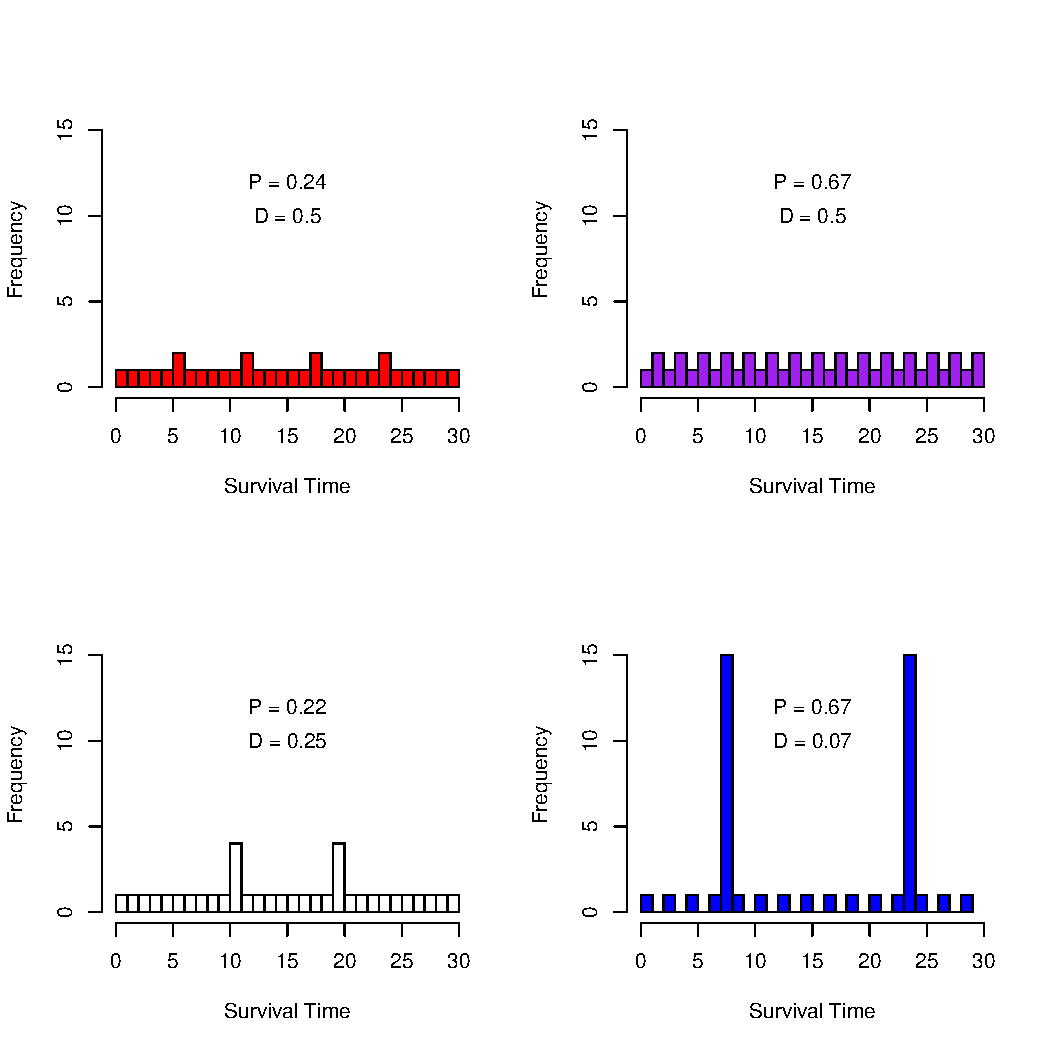
\includegraphics{HistogramIllustrations.pdf}} \\
        \resizebox{7.75in}{!}{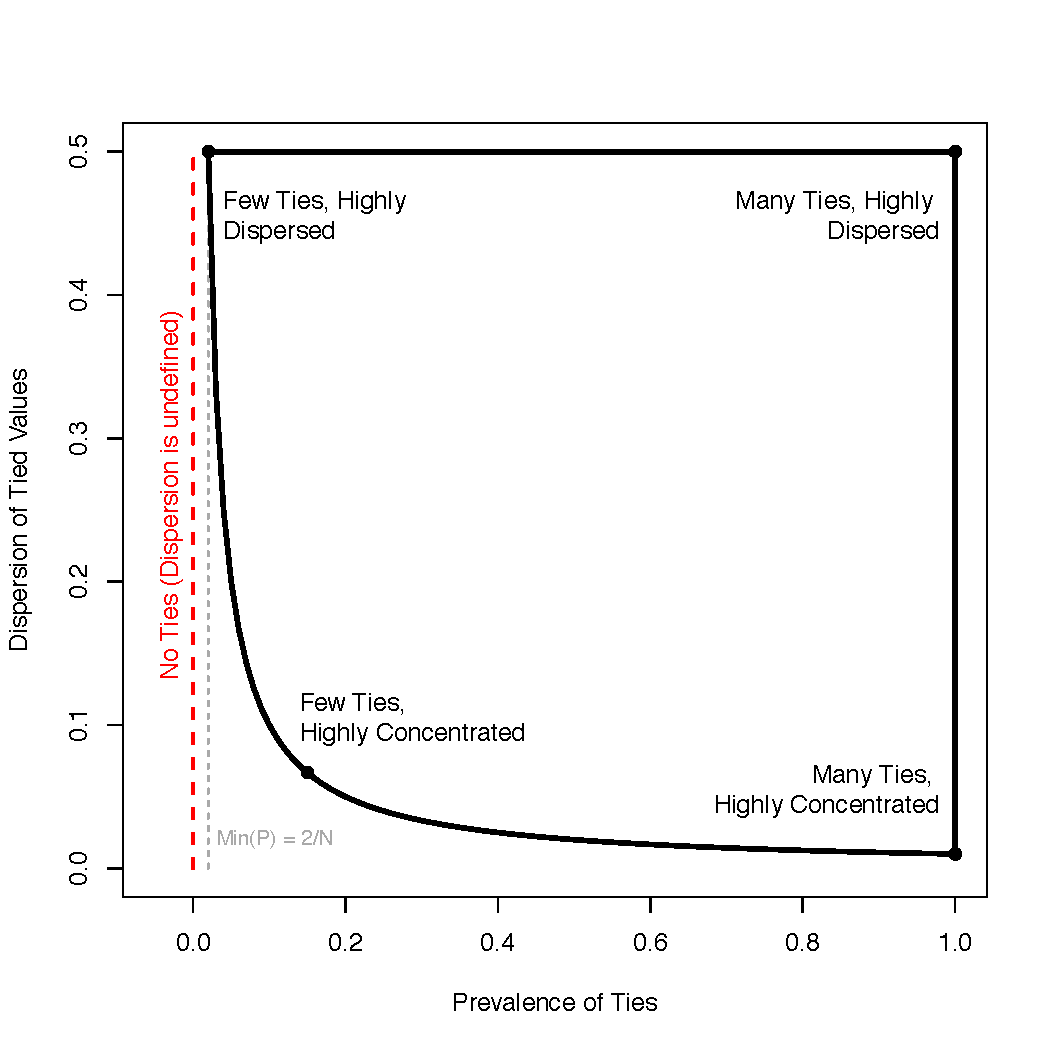
\includegraphics{PvsDConceptualPlot.pdf}}
        \end{center}
        \end{figure}
      \end{block}

    \end{column}%2

    %-- Column 3 ---------------------------------------------------
    \begin{column}{0.24\linewidth}


      %-- Block 3-1
      \begin{block}{Simulation Procedure}
      \noindent Exponential survival times:
               \begin{align*}
               T_{i} = \text{Exponential}(0 + 1.0 X_{i})       &  & N \in \{60,600,6000\} \\
                X_{i} \sim i.i.d.\ \text{Bernoulli}(0.5)            & & P \in [0.2,1]  \\
                                                                                   & & D \in [0.1,0.5]
          \end{align*}
      \begin{itemize}
      \item ``Jitter'': adding $\lambda=1000$ exponential noise to each observation.
      \item $K = 1000$ replications for each permutation of $\{N,P,D\}$
      \item $\text{Percent Absolute Bias}_{N,P,D} = \left| \frac{\sum_{k=1}^{K} \hat{\beta}_{k} - 1}{1000} \right| \times 100$
      \end{itemize}
      \end{block}


      %-- Block 2-2
      \begin{block}{Simulation Results}

        \begin{figure}[h]
        \begin{center}
        Percent Absolute Bias in $\hat{\beta}$, $N=60$ \\
        %\caption{Prevalence and Dispersion} \label{POLMETHFigOne} \\
        \resizebox{9in}{!}{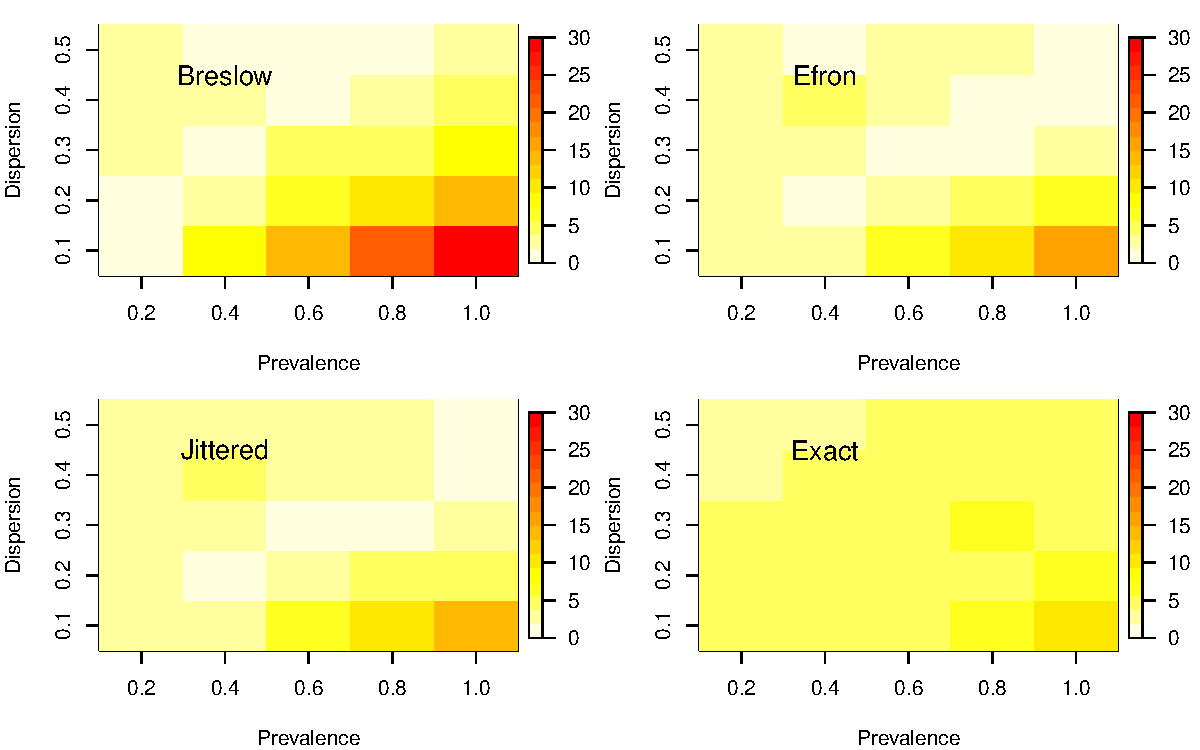
\includegraphics{AbsBias60.pdf}}
        \end{center}
        \end{figure}

        \begin{figure}[h]
        \begin{center}
        Percent Absolute Bias in $\hat{\beta}$, $N=600$ \\
        %\caption{Prevalence and Dispersion} \label{POLMETHFigOne} \\
        \resizebox{9in}{!}{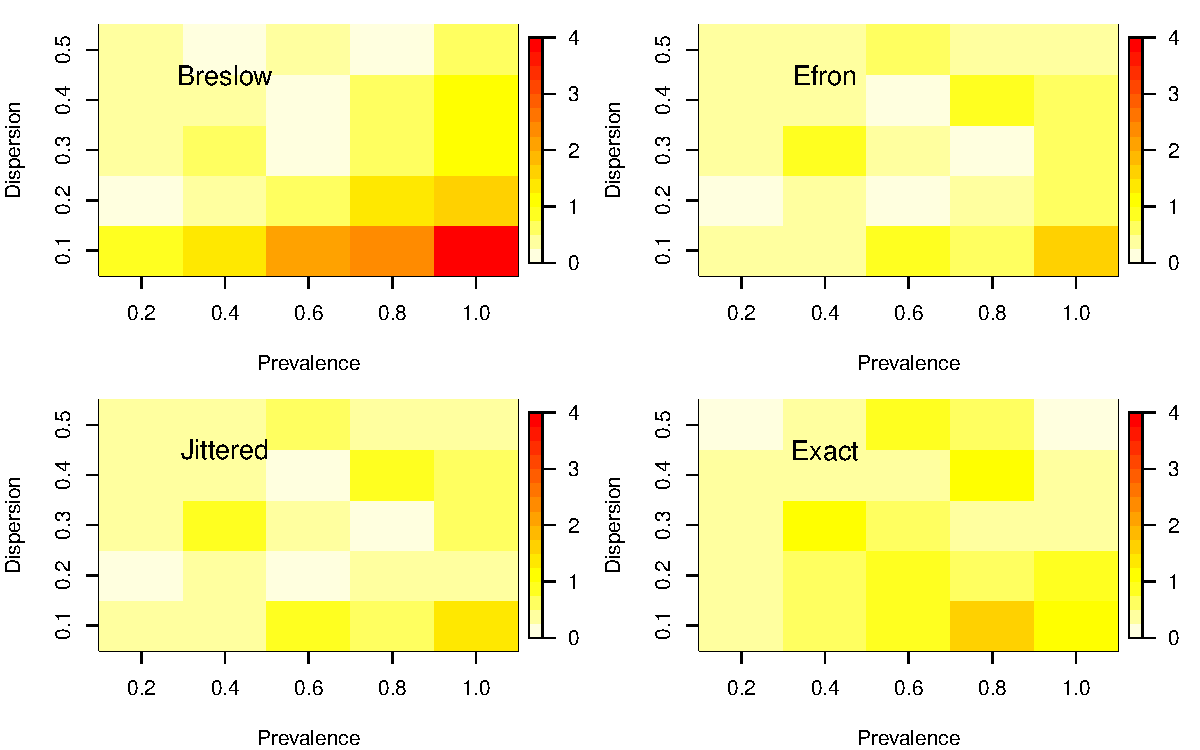
\includegraphics{AbsBias600.pdf}}
        \end{center}
        \end{figure}

        \begin{figure}[h]
        \begin{center}
        Percent Absolute Bias in $\hat{\beta}$, $N=6000$ \\
        %\caption{Prevalence and Dispersion} \label{POLMETHFigOne} \\
        \resizebox{9in}{!}{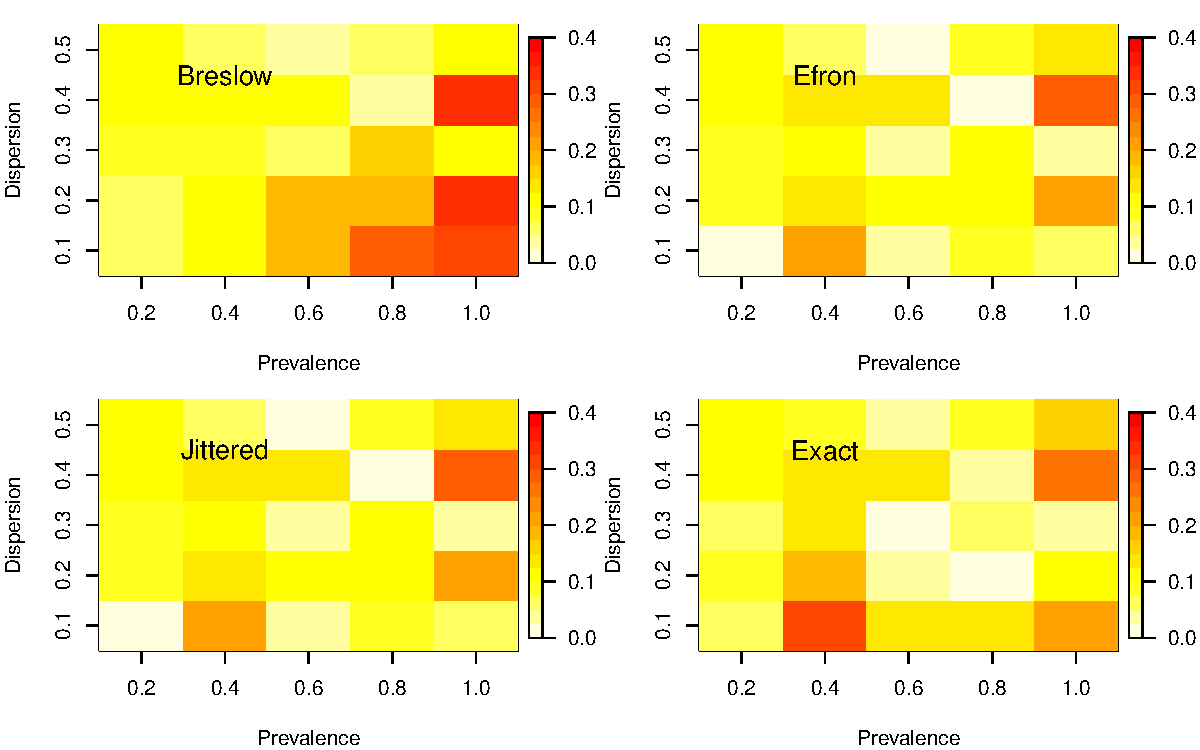
\includegraphics{AbsBias6000.pdf}}
        \end{center}
        \end{figure}

      \end{block}

    \end{column}%3

    %-- Column 4 ---------------------------------------------------
    \begin{column}{0.24\linewidth}

      %-- Block 3-1
      \begin{block}{Existing Studies}
      \begin{itemize}
      \item Existing studies in political science are characterized by high tie prevalence and varying levels of dispersion.
      \item In general, higher tie prevalence is associated with lower dispersion / greater concentration of ties among a few values.
      \end{itemize}

        \begin{figure}[h]
        \begin{center}
        %\caption{Prevalence and Dispersion} \label{POLMETHFigOne} \\
        \resizebox{10in}{!}{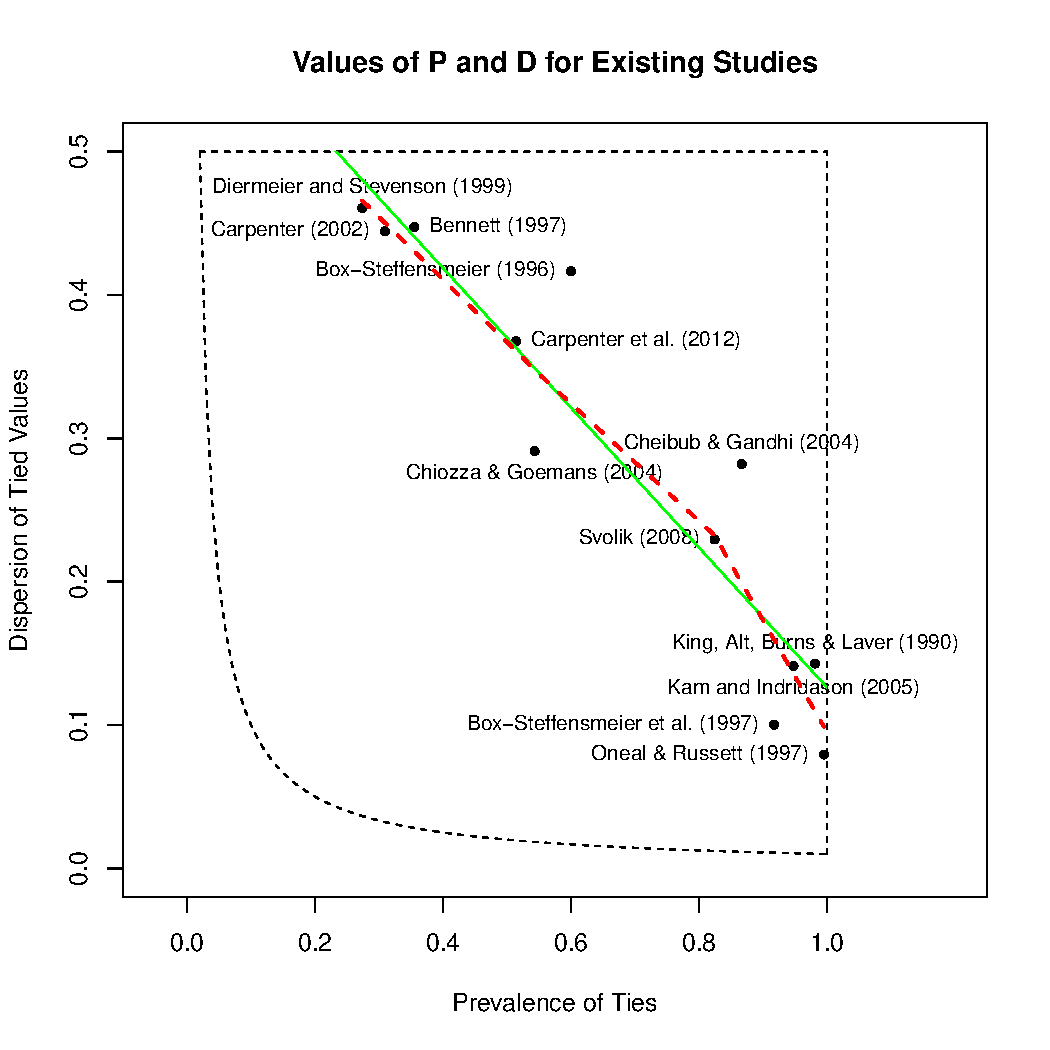
\includegraphics{PvsDRealStudies.pdf}}
        \end{center}
        \end{figure}


      \end{block}

      %-- Block 3-2
      \begin{block}{Implications and Future Work}

      \noindent {\bf Implications} \\

      \begin{itemize}
      \item All methods perform equally well when $P < 0.5$.
      \item For $P > 0.5$, all methods perform equally well if dispersion is high (i.e., when there are large numbers of survival times with relatively few tied observations per time).
      \item If $P$ is high and $D$ is low, the exact method is strongly recommended.
      \item For all approximations, the degree of bias decreases in the sample size at roughly $O(1/N)$.
      \end{itemize}

      \noindent {\bf Future Work} \\

      \begin{enumerate}
      \item Examine standard error estimates and effective coverage rates.
      \item Assess sensitivity to ``asymmetrically'' tied data.
      \item Develop simple R and Stata routines to aid model selection.
      \end{enumerate}

      \end{block}

 %-- Block 3-2
      \begin{block}{References}

      \noindent Cox, D.R.  1972.  ``Regression Models and Life Tables.''  \emph{Journal of the Royal Statistical Society, Series B} 34(2): 187-220. \\

       \noindent Efron, Bradley (1974). ``The Efficiency of Cox's Likelihood Function for Censored Data.'' \emph{Journal of the American Statistical Association} 72 (359): 557-565. \\

       \noindent Hertz-Picciotto, Irva, and Beverly Rockhill.  1997. ``Validity and Efficiency of Approximation Methods for Tied Survival Times in Cox Regression.''  \emph{Biometrics} 53(3):1151-1156.

       \end{block}

    \end{column}%4

  \end{columns}
\end{frame}


\end{document}
